\chapter{Evaluation}
\label{sec:eval}

\section{Simulation Model} 

% Mitzenmacher suggested in his thesis \cite{mitzenmacher1996power} that researchers who work with load balancing models should pair their theoretical analyses with numerical results and simulations. The reason for this pairing is to provide clear indications of the significance of the results in order to make these results accessible to practitioners. I take inspiration and direction from Mitzenmacher's suggestions in this chapter of my thesis where I expound on the results of my experiments run through a custom built simulator. 

Before considering details of the simulation experiments, we formalize the simulation model and how it applies to the needle algorithm proxy distribution strategy. The notion of static and dynamic models stems from static and dynamic routing in networks. Mitzenmacher redefined static and dynamic models for task allocation and applied this to the balls and bins model \cite{mitzenmacher1996power}. In this context, a ball is a task and a bin is a processor. The primary distinguishing features of the static model is that there are a finite number of tasks that are assigned to processors and these tasks do not leave. The static system model completes its execution when all of the tasks are allocated. This model execution is generally represented in a bipartite graph. A static model applied to the proxy distribution problem assigns a finite number of clients to proxies in one round.

The dynamic model captures scenarios that are more realistic than what may be represented in the static model. For example, tasks in the dynamic model may enter and leave the system over time. In the open dynamic model, there may not be a fixed number of tasks. The closed dynamic model allows for tasks to enter and leave over time, but there is a fixed number of arrivals. A dynamic system does not have a final termination time as in the static model. The advantage of a dynamic model is that one can observe the behaviour of a system over time.

We are interested in how proxies are enumerated by a censor throughout the system's lifetime, so the open dynamic model suits our scenario well. Utilizing an open dynamic model allows us to observe trends and compare different approaches temporally.

In addition to the dynamic model, the queue model is a standard that suits the problem of proxy distribution well. Mitzenmacher models the power of two choice algorithm as an idealized process, or a queue system of infinite size, that is later related to a finite system by bounding the error between the two \cite{mitzenmacher1996power}. 

Our simulation is best described as a feed-forward network of M/M/c/k queues. This is similar to a load balancing system with a constant number of servers. However, in this scenario, the load balancer is in fact the proxy distributor that is responsible for distributing clients to proxies. The number of proxies is fixed; their respective enumerations represent a pure death process, as I do not consider proxy birth rate in the system. Figure \ref{fig:mmck} shows the network queue layout where the proxy distributor assigns clients to proxies uniform randomly, where the arrival of clients to proxies is evenly distributed $\lambda/n$. 

%%%%%%%%%%%%%%%%%%%%%%%%%%%%%%%%%%%%%%%%%%%%%%%%%%%%%%%%%%%%%%%%%%%%%%
\begin{figure*}[h!]
\centering
     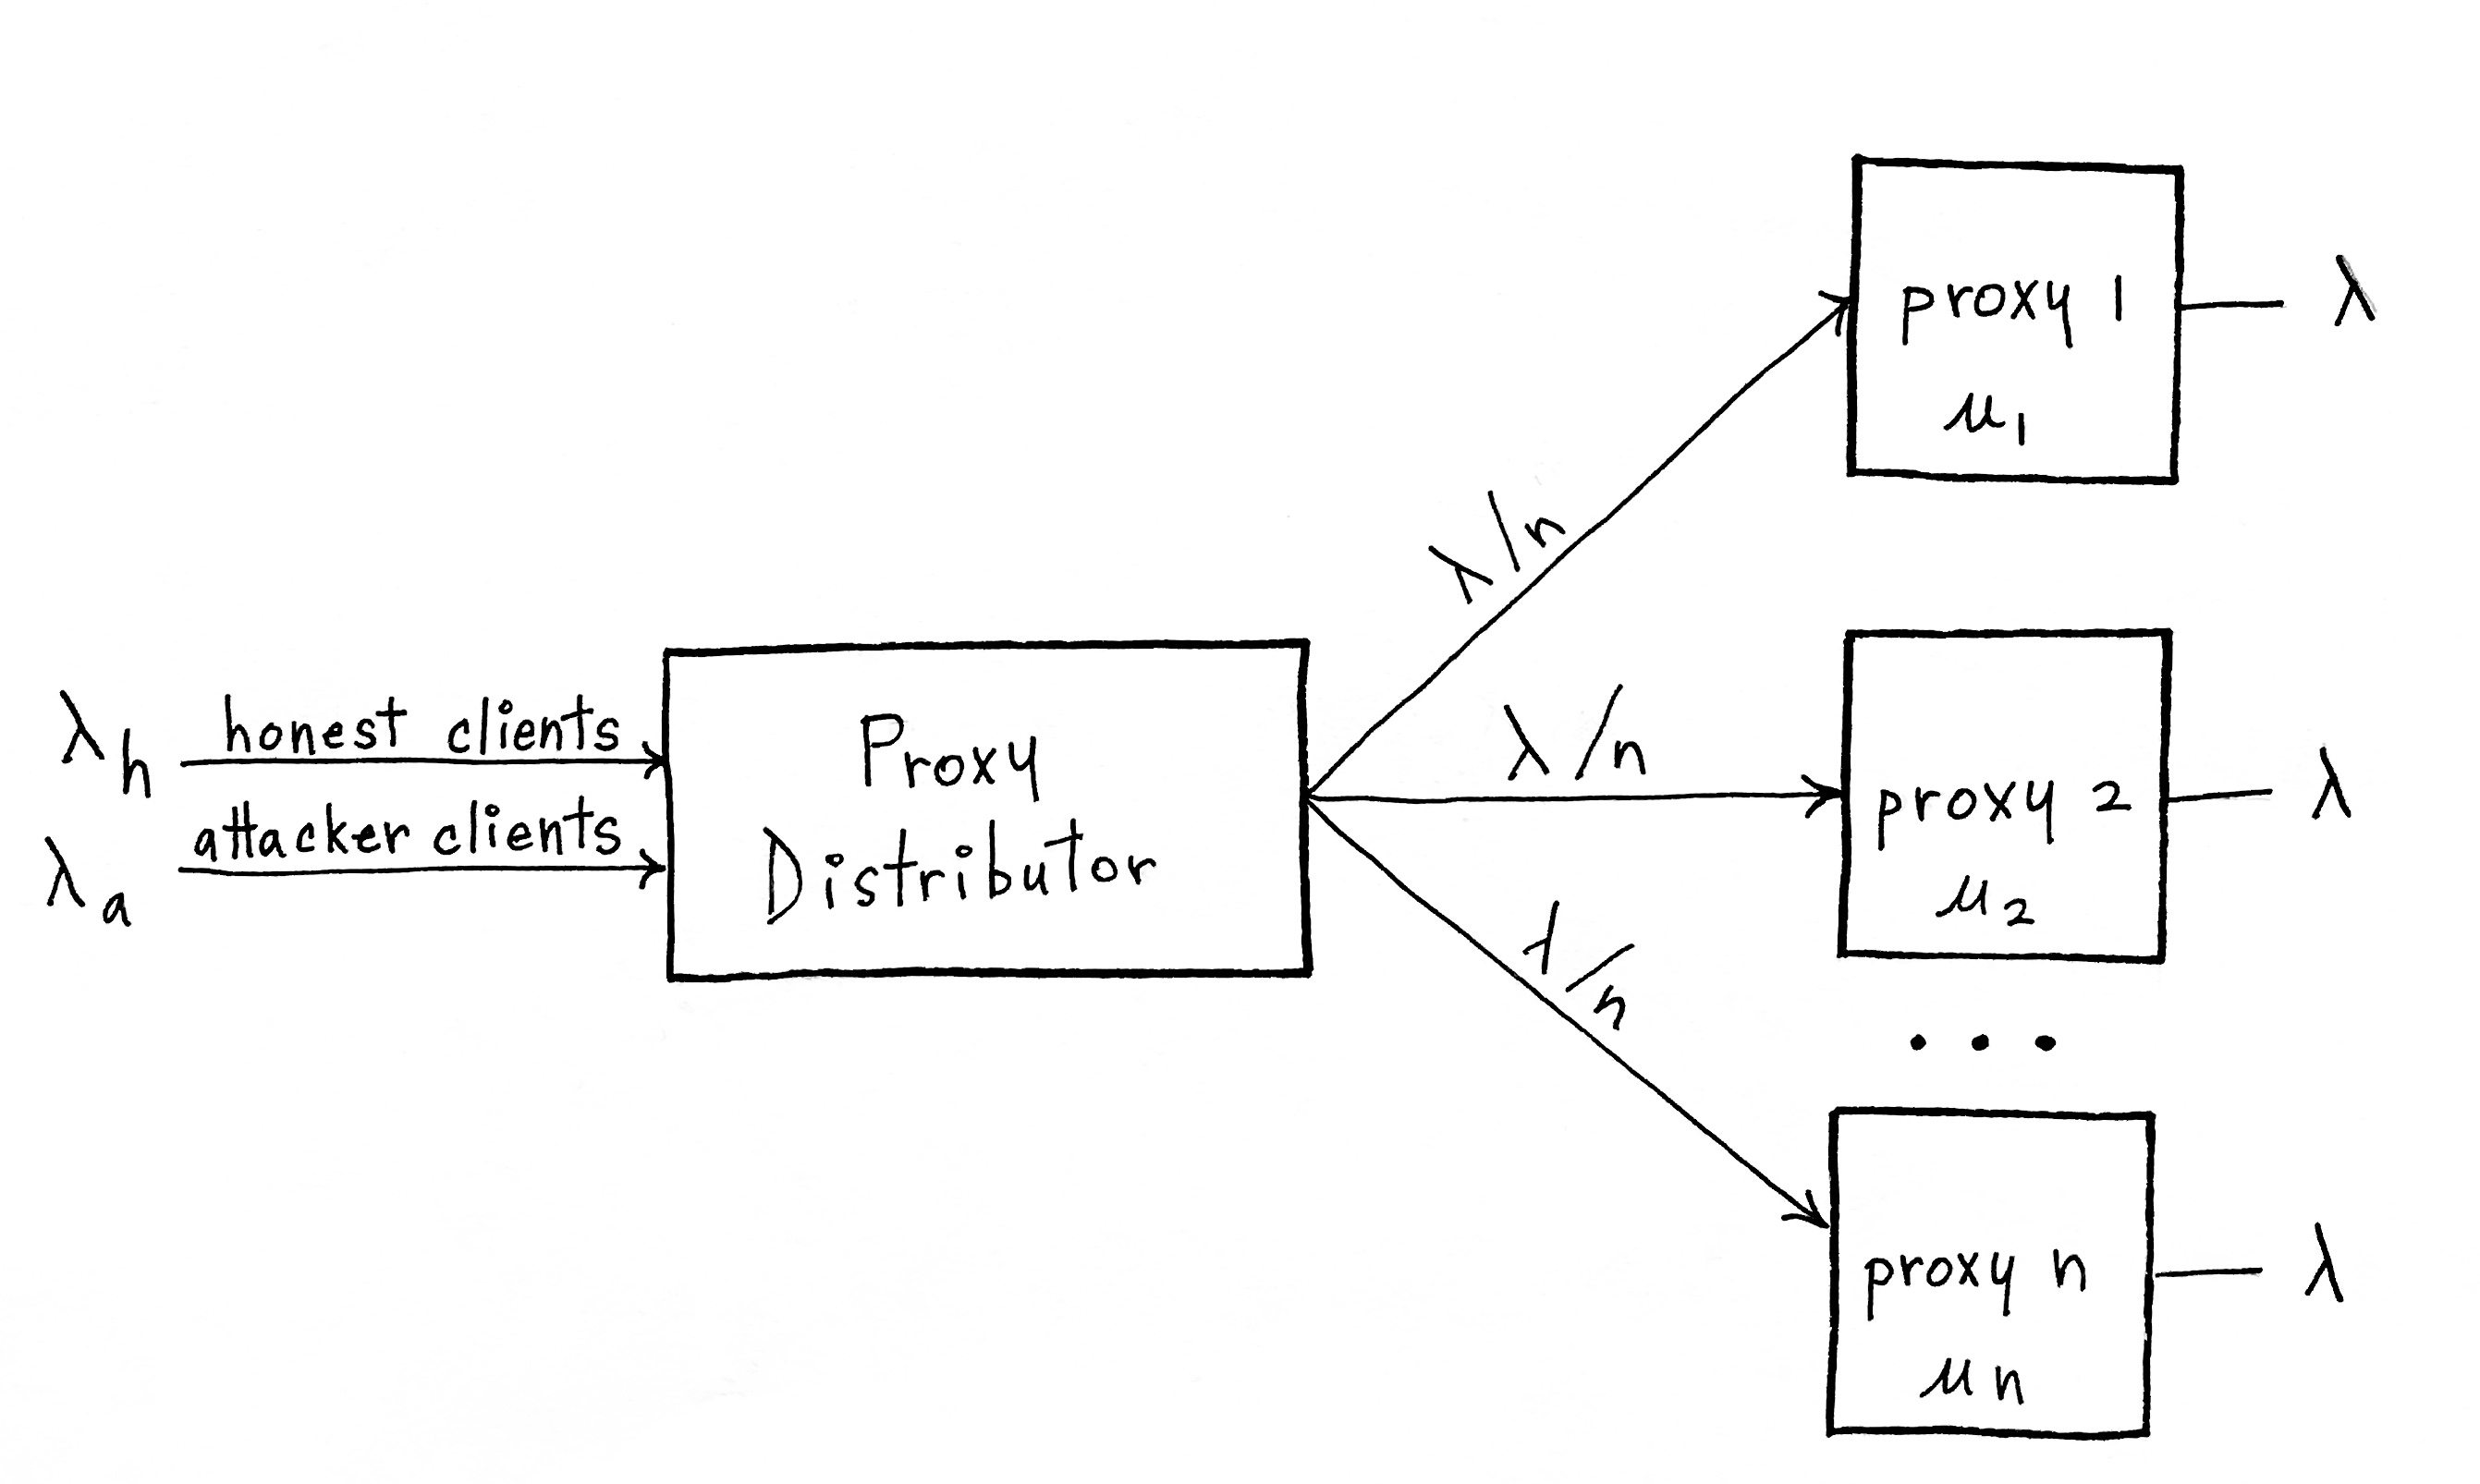
\includegraphics[width=1.0\textwidth]{fig/mmck_queue.png}
    \caption{M/M/c/k with uniform random distribution}

    \label{fig:mmck}
\end{figure*}
%%%%%%%%%%%%%%%%%%%%%%%%%%%%%%%%%%%%%%%%%%%%%%%%%%%%%%%%%%%%%%%%%%%%%%

Clients arrive with a Poisson arrival distribution with variable $\lambda$ clients per minute. This means that, on average, one client appears at every $1 / \lambda$ minutes and we define this as the arrival intensity. In this model, we are additionally concerned with honest and malicious client arrival rates. As the proportion of attackers in the system increases, the arrival rate, or intensity of malicious client arrivals increases.
% TODO define the needle case probability lambda/?, this belongs in the probabilistic analysis above

Each proxy has an service time that is exponentially distributed. This is not a traditional service rate because the system assumes short-lived client connections. The important function of the server is to keep a record of each client assignment that can be used by the censor to discover clients in the system. In other words, even if the client leaves the system, the censor still gains knowledge of the proxy and may affect the client's future connections to the known proxy, effectively mounting a potential future blocking attack on the client, as well as the proxy.

% no longer seems applicable
%We define the aggressive blocking strategy as a censor that blocks each proxy as it is discovered. A complete blocking strategy is a simplified version of delayed blocking where the censor blocks all of the proxies when they are all enumerated, with the assumption that the censor knows the total number of proxies in the system in order to simplify the analysis. The choice of model here is important because it informs the behaviours of an attacker. 

\textbf{Parameters.} Parameters in the simulation control the rate of honest and malicious client arrival intensity, the total number of proxies, and the size of the sliding window for the needle algorithm. These are sweeping parameters; the simulation runs across a range of values for each parameter to produce a variety of conditions for the analysis. The analysis operates on the dependent variables such as maximum load and the expected time to overtake the system. The variable names and descriptions are outlined in the following table:

\begin{table}[h]
  \centering
	\begin{tabular}{ll}
	\hline
	\cline{1-2}
	Parameter Name   & Description  \\
	\hline
    CLIENT ARRIVAL RATE & intensity of client arrival rate \\
	ATTACKER ARRIVAL RATE      & sigma for client arrival rate \\
	NUM PROXIES      & sigma for blocking rate \\
	\hline
	\end{tabular}
  \caption{Variables in the Simulation}
  \label{tab:vars}
\end{table}

The simulator was written in Python using simpy, a discrete event based simulator.\footnote{https://simpy.readthedocs.io/en/latest/} The evaluation uses numpy\footnote{http://www.numpy.org/} and matplotlib\footnote{https://matplotlib.org/} for data manipulation and graphing.

\section{Enumeration Results}

\textbf{Giant step analysis.} We ran the needle algorithm in the simulator, with only malicious attacker clients, to observe how many assignments a censor needs to enumerate all of the proxies. In section \ref{UBGS}, we analyzed the giant step version of the needle algorithm where step size $g > 1$. Asymptotic results are shown in Figure \ref{fig:gsn100} for 1000 trials using 100 proxies in each experiment. The experimental results are shown in the black, solid line. The upper and lower bounds, $E[X] \leq \frac{(n^2)H_{\lceil{H_n}\rceil}}{g}$ and $E[X] \geq (g)(s^2H^{(2)}_{\lfloor{H_n}\rfloor})$ respectively, are shown in dashed lines.

%%%%%%%%%%%%%%%%%%%%%%%%%%%%%%%%%%%%%%%%%%%%%%%%%%%%%%%%%%%%%%%%%%%%%%
\begin{figure*}[h!]
\centering
     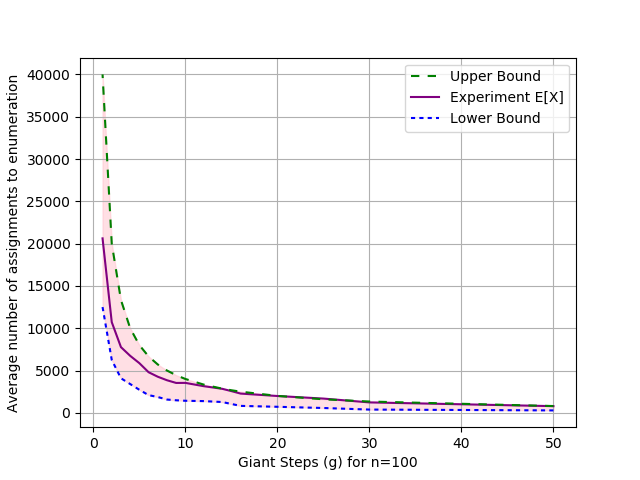
\includegraphics[width=1.0\textwidth]{fig/needle_expected_value_n_100.png}
    \caption{Giant step enumeration comparison for 100 proxies}

    \label{fig:gsn100}
\end{figure*}
%%%%%%%%%%%%%%%%%%%%%%%%%%%%%%%%%%%%%%%%%%%%%%%%%%%%%%%%%%%%%%%%%%%%%%

\textbf{Enumeration Comparison.} We know from the Coupon Collector problem that the uniform random distribution of coupons results in $nH_n$ total assignments before collection. We see that the uniform random distribution of Tor's \texttt{bridgedb} follows a similar enumeration. We use the regular Power of 2 Choices algorithm to show how a more optimal load balancing algorithm results in faster enumeration\cite{xu2011generalized}. In the upcoming section, we'll take a closer look at the load balancing properties of each of these algorithms.

%%%%%%%%%%%%%%%%%%%%%%%%%%%%%%%%%%%%%%%%%%%%%%%%%%%%%%%%%%%%%%%%%%%%%%
\begin{figure*}[h!]
\centering
     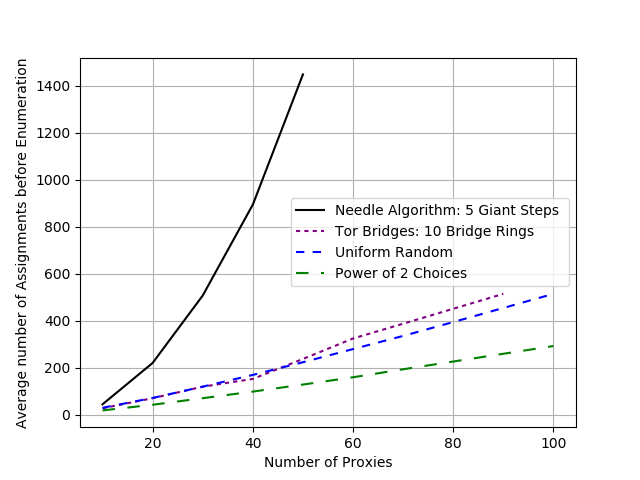
\includegraphics[width=1.0\textwidth]{fig/comparison_graph.png}
    \caption{Enumeration comparison}

    \label{fig:comparison}
\end{figure*}
%%%%%%%%%%%%%%%%%%%%%%%%%%%%%%%%%%%%%%%%%%%%%%%%%%%%%%%%%%%%%%%%%%%%%%

\section{Load Balancing Results}

We observe the needle's load balancing tendencies where the total number of proxies is $n$. Figure \ref{fig:needlelb1} shows the number of proxies sorted by their respective load on the x-axis. The y-axis shows the percentage of the total load that each proxy holds. The maximum load for each of the experiments is no more than 5\% of the total load. This experiment terminates when there are $n$ assignments, so that we can compare our results to known balls-in-bins bounds, shown in Figure \ref{fig:compare1}.

%%%%%%%%%%%%%%%%%%%%%%%%%%%%%%%%%%%%%%%%%%%%%%%%%%%%%%%%%%%%%%%%%%%%%%
\begin{figure*}[h!]
\centering
     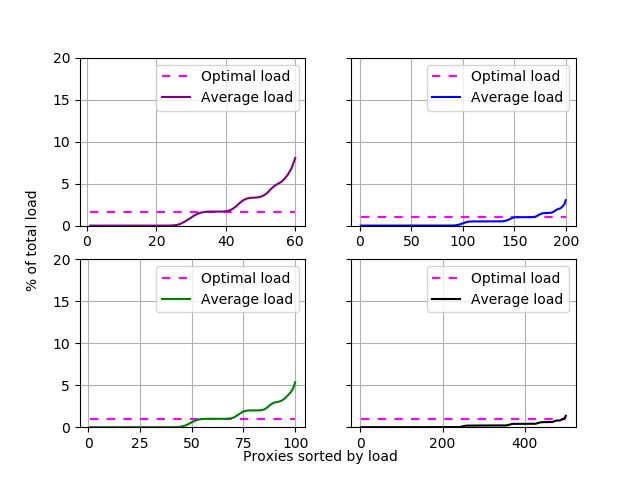
\includegraphics[width=1.0\textwidth]{fig/load_balance_needle_to_n_60_100_200_500.png}
    \caption{Needle Load Balancing where $m=n$ for $n=60, 100, 200, 500$.}

    \label{fig:needlelb1}
\end{figure*}
%%%%%%%%%%%%%%%%%%%%%%%%%%%%%%%%%%%%%%%%%%%%%%%%%%%%%%%%%%%%%%%%%%%%%%


A distinguishing feature of each algorithm is their varying degree of even distribution of assignments to proxies. The power of two choices algorithm gives the most evenly balanced distribution. The uniform random distribution results in the next best load balancing. At the other end of the load balancing spectrum, the $needle$ algorithm results in the worst load balancing.

%%%%%%%%%%%%%%%%%%%%%%%%%%%%%%%%%%%%%%%%%%%%%%%%%%%%%%%%%%%%%%%%%%%%%%
\begin{figure*}[h!]
\centering
     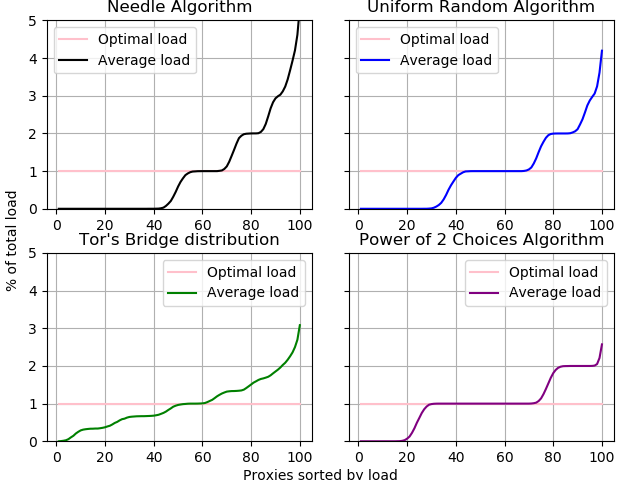
\includegraphics[width=1.0\textwidth]{fig/load_balance_comparison_to_n_100.png}
    \caption{Comparison Load Balancing where $m=n$}

    \label{fig:compare1}
\end{figure*}
%%%%%%%%%%%%%%%%%%%%%%%%%%%%%%%%%%%%%%%%%%%%%%%%%%%%%%%%%%%%%%%%%%%%%%

% TODO what is the maximum load and is it the correct bound loglogn/logn?

%%%%%%%%%%%%%%%%%%%%%%%%%%%%%%%%%%%%%%%%%%%%%%%%%%%%%%%%%%%%%%%%%%%%%%
\begin{figure*}[h!]
\centering
     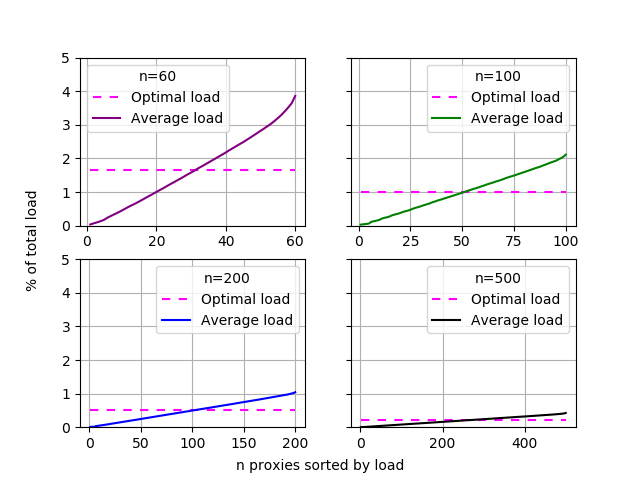
\includegraphics[width=1.0\textwidth]{fig/load_balance_needle_to_twice_enum_60_100_200_500.png}
    \caption{Needle Load Balancing until all proxies are enumerated twice for $n=60, 100, 200, 500$.}

    \label{fig:needlelb2}
\end{figure*}
%%%%%%%%%%%%%%%%%%%%%%%%%%%%%%%%%%%%%%%%%%%%%%%%%%%%%%%%%%%%%%%%%%%%%%


In the experiments shown in Figure \ref{fig:needlelb2}, we ran the needle trials until all of the proxies were enumerated and then kept running the trials until twice the number of enumeration time. Here we see the analysis from Lemma $9$ in section \ref{sec:lb} where $px_{n/2}$ has the optimal load. We see that the load balancing continues to become more divided into two halves centred around the optimal load. 


\section{Bystander Results}

Our bystander results are affected by load balancing and the proportion of attackers in the simulation. For the experiment in Figure \ref{fig:bystandercompare}, we run all of the algorithms so they all have 2000 assignments. We sort the proxies by their loads increasing and show the numbers of malicious attackers assigned to each proxy, from lowest loaded to highest.

%%%%%%%%%%%%%%%%%%%%%%%%%%%%%%%%%%%%%%%%%%%%%%%%%%%%%%%%%%%%%%%%%%%%%%
\begin{figure*}[h!]
\centering
     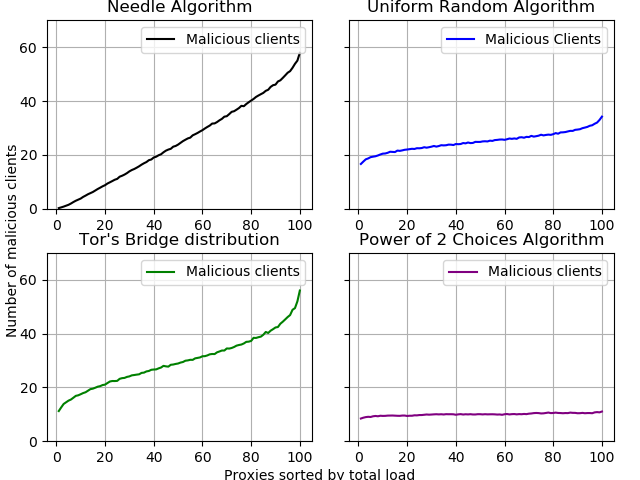
\includegraphics[width=1.0\textwidth]{fig/bystander_comparison_to_n_100.png}
    \caption{Comparison of Malicious Clients}

    \label{fig:bystandercompare}
\end{figure*}
%%%%%%%%%%%%%%%%%%%%%%%%%%%%%%%%%%%%%%%%%%%%%%%%%%%%%%%%%%%%%%%%%%%%%%

We see from the results of this experiment that the number of malicious attackers is increased with load in all of the algorithms, however, in the needle algorithm, lighter loaded proxies have fewer malicious clients. The power of 2 choices algorithm has the flattest distribution of malicious clients, meaning that proxies are enumerated the quickest.

\todo{Graph showing the average total number of bystanders over all experiments (capped at 2000 assignments}


\section{Comparison}

We consider enumeration, load balancing, and bystanders analyses of the four algorithms in order to contrast their respective trade-offs and suitability under differing system goals. Table \ref{tab:tradeoff} outlines the three metrics that we consider in this thesis. We indicate with checkmarks \ding{51} where the algorithm is well suited, double checkmarks indicate that it is very well suited. A single X mark \ding{55} shows that the algorithm is unsuitable, a double \ding{55}  is used when we consider the algorithm to be completely unusable for a purpose.

The Power of 2 Choices algorithm provided the best load balancing, and so would be appropriate for systems where this is a concern. However, it is also enumerated very quickly and has the highest amount of bystanders.

Uniform random distribution and Tor's \texttt{bridgedb} distribution perform similarly, and so we consider their respective trade-offs in the same vein. They provide a slower enumeration time than the Power of 2 Choices algorithm, however, this is due to unevenness in the load balancing. The number of bystanders is not as drastic a drawback as with Power of 2 Choices, but it is not as good as with the Needle algorithm. 

The Needle algorithm gives the slowest enumeration of all the algorithms; this attribute is beneficial to allocation of proxies in a distribution system. It is not suitable for systems that require even load balancing. (It is unbalanced to a large degree but not so much that it is unusable.) Its lower number of bystanders is due to its relatively uneven load balancing. In the context of proxy distribution under our threat model, we consider this a benefit.

\begin{table}[t]
\begin{tabular}{l*{3}{|c}r}
             & Enumeration & Load Balancing & Bystanders \\
\hline
\hline
Power of 2 Choices & \ding{55}\ding{55}  & \ding{51}\ding{51} & \ding{55}\ding{55} \\
Uniform            & \ding{55}  & \ding{51} & \ding{55}  \\
Tor's \texttt{bridgedb} & \ding{55}  & \ding{51} & \ding{55}  \\
Needle           & \ding{51}\ding{51}  & \ding{55}\ding{55}  & \ding{51}\ding{51}  \\
\end{tabular}
\caption{Comparison chart of the 4 algorithms\label{tab:tradeoff} }
\end{table}